\documentclass{article}

%----------------------------------------------------------------------------------------
%	Packages
%----------------------------------------------------------------------------------------
\usepackage[utf8]{inputenc}	% für Umlaute ect.
\usepackage{fancyhdr} % für header
\usepackage{lastpage} % für footer
\usepackage{extramarks} % für header und footer
\usepackage{amsthm} % math stuff
\usepackage{amsmath} % math stuff
\usepackage{amssymb} % math stuff
\usepackage{color}
\usepackage{listings} % code listings
\usepackage{enumitem}
\usepackage{graphicx} % für graphics
\usepackage{caption}
\usepackage{subcaption}
\usepackage{multicol}
\usepackage{pgf}
\usepackage{tikz}
\usetikzlibrary{arrows,automata}

%------------------------------------------------------------------
%	Allegmeine Dokumentsettings
%------------------------------------------------------------------
% Margins
\topmargin=-0.45in
\evensidemargin=0in
\oddsidemargin=0in
\textwidth=6.5in
\textheight=9.0in
\headsep=0.25in

%Header und Footer
\pagestyle{fancy}
\chead{\moduleTitle}  
\rhead{}
\lfoot{\lastxmark}
\cfoot{} 
\rfoot{\ \thepage\ of\ \protect\pageref{LastPage}}
\renewcommand\headrulewidth{0.4pt} % Size of the header rule
\renewcommand\footrulewidth{0.4pt} % Size of the footer rule

% Zeilenabstand
\linespread{1.0} 

%----------------------------------------------------------------------------------------
%	Commands and Environments
%----------------------------------------------------------------------------------------

\newcommand{\moduleTitle}{Graph Bisections}


% Für Code listings
\lstset{ %
	language=Python,                % choose the language of the code
	basicstyle=\footnotesize,       % the size of the fonts that are used for the code
	numbers=left,                   % where to put the line-numbers
	numberstyle=\footnotesize,      % the size of the fonts that are used for the line-numbers
	stepnumber=1,                   % the step between two line-numbers. If it is 1 each line will be numbered
	numbersep=5pt,                  % how far the line-numbers are from the code
	backgroundcolor=\color{white},  % choose the background color. You must add \usepackage{color}
	showspaces=false,               % show spaces adding particular underscores
	showstringspaces=false,         % underline spaces within strings
	showtabs=false,                 % show tabs within strings adding particular underscores
	frame=single,           % adds a frame around the code
	tabsize=2,          % sets default tabsize to 2 spaces
	captionpos=b,           % sets the caption-position to bottom
	breaklines=true,        % sets automatic line breaking
	breakatwhitespace=false,    % sets if automatic breaks should only happen at whitespace
	escapeinside={\%*}{*)}          % if you want to add a comment within your code
}

% An environment for stpes, cases ect. 
% From: http://tex.stackexchange.com/questions/32798/a-step-by-step-environment
\newenvironment{steps}[1]{\begin{enumerate}[label=#1 \arabic*]}{\end{enumerate}}
\makeatletter%
\def\step{%
	\@ifnextchar[ \@step{\@noitemargtrue\@step[\@itemlabel]}}
\def\@step[#1]{\item[#1]\mbox{}\\\hspace*{\dimexpr-\labelwidth-\labelsep}}
\makeatother

%-----------------------------------------------------------------------------
%	Theoreme
%-----------------------------------------------------------------------------
\newtheorem{mydef}{Definition}
\newtheorem{mybei}{Beispiel}
\newtheorem*{mybei*}{Beispiel}
\newtheorem{mysatz}{Satz}
\newtheorem*{mysatz*}{Satz}
\newtheorem{mybew}{Beweis}
\newtheorem*{mybew*}{Beweis}
\newtheorem{myfolg}{Folgerung}
\newtheorem*{myfolg*}{Folgerung}
\newtheorem{mybemerk}{Bemerkung}
\newtheorem*{mybemerk*}{Bemerkung}

\begin{document}
	\section{Spektrale Graph Bisektion}
\subsection{Idee}
\begin{itemize}
	\item Formuliere Graph-Partition als diskretes Optimierungsproblem
	\item Ersetzte dieses durch ein kontinuierliches Optimierungsproblem
\end{itemize}

\subsection{Integer Linear Programm}
\begin{mydef}
	Laplace-Matrix \\
	die Laplace-Matrix $L(G)$ eines Graphen $G=(V,E)$ ist eine $|V|*|V|$ symmetrische Matrix, wobei gilt:
	$$
	L(G)(i,j)=
	\begin{cases}
	\text{Knotengrad von } v_i & i=j,\\
	-1 & i\not=j \\
	0 & sonst
	\end{cases}
	$$
\end{mydef}

\begin{mysatz*}
	Satz von Fiedler (1975) \\
	Sei $G=(V,E)$ ein Graph, $V=V_1 \cup V_2$ eine beliebige Partition mit $|V| = n$, der Laplace Matrix $L(G)$ und einem Indexvektor $x$ mit:
		$$
		x_i=
		\begin{cases}
		1 & v_i \in V_1\\
		-1 & v_i \in V_2 
		\end{cases}
		$$
	Dann gilt:
	\begin{center}
		Die Anzahl der Kanten zwischen $V_1$ und $V_2$ beträgt $\frac{1}{4}x^TL(G)*x$
	\end{center}
\end{mysatz*}

Im Folgenden gelte: $z \in \{0,1\}^n$

\begin{mybew*}
	Schritt 1 \\
	Sei $A$ die Adjazenmatrix von $G$, dann gilt:
	\begin{flalign*}
		z^TAz = & \sum\limits_{i,j}a_{ij}z_iz_j \\
		= & 2\sum\limits_{i,j (i,j)\in E} z_iz_j  \\
		= & 2*(-|\text{Schnittkanten}| + |E| - |\text{Schnittkanten}|) \\
		= & -2|E| + 4|Schnittkanten|
	\end{flalign*}
	Beachte hierzu:
	\begin{flalign*}
	z_iz_j = 
	\begin{cases}
		1 & (i,j) \not \in \text{Schnittkanten}  \\
		-1 & (i,j) \in \text{Schnittkanten}
	\end{cases}
	\end{flalign*}
	Und:
	\begin{center}
		$z_j*a_ij*z_i = 0 \Leftrightarrow a_{ij} =0$ \\
		$\Rightarrow$ Es gibt keine Kanten von $i$ nach $j$
		
	\end{center}
	Das heißt uns interessiert nur der Fall, in dem $(i,j) \in E$
\end{mybew*}
\begin{mybew*}
	Schritt 2 \\
	Sei $D$ die degree-Matrix von $G$. Dann gilt:
	\begin{flalign*}
		z^TDz = & \sum\limits_{i,j}d_{ij}z_iz_j \\
		= & \sum\limits_{i} d_{ii} = 2*|E|
	\end{flalign*}
	Beachte: Die Summe der Diagonaleinträge entspricht der doppleten Anzahl der Kanten in $G$!
	\begin{flalign*}
	z_id_{i,j}z_j = 
	\begin{cases}
			0 & i \not = j \\
			d_{i,j} & sonst
	\end{cases}
	\end{flalign*} 
\end{mybew*}
\begin{mybew}
	Schritt 3 \\
	Sei $A$ die Adjazenzmatrix, $D$ die Diagonalmatrix und $L$ die Laplacematrix, wobei $L = D-A$ \\
	Dann gilt:
	\begin{flalign*}
		\frac{1}{4}(z^TDz - z^TAz) = |\text{Schnittkanten}| \\
		\Rightarrow \frac{1}{4}(z^TLz) = |\text{Schnittkanten}|
	\end{flalign*} 
\end{mybew}

Alternative Herleitung:
\begin{mybew*}
	\begin{flalign*}
		x^TL(G)x &= \sum\limits_{i,j} L(G)(i,j)x_ix_j  \\
		 &= \sum\limits_{i=j} L(G)(i,j)x_i^2  + \sum\limits_{i\not = j}L(G)(i.j)x_ix_j \\
		 &= \sum\limits_{i=j} L(G)(i,j)x_i^2  + \sum\limits_{i\not = j,i,j\in V_1}L(G)(i.j)x_ix_j + \sum\limits_{i\not = j,i,j\in V_2}L(G)(i.j)x_ix_j + \sum\limits_{i\not = j,i\in V_1,j\in V_2}L(G)(i.j)x_ix_j \\
		 &= \sum\limits_{i}grad(i)+ \sum\limits_{i\not = j,i,j\in V_1}(-1)(+1)(+1) + \sum\limits_{i\not = j,i,j\in V_2}(-1)(-1)(-1) + \sum\limits_{i\not = j,i\in V_1,j\in V_2}(-1)(+1)(-1) \\
		 &= 2*|E| - 2*|E_{(V_1,V_1)}| - 2*|E_{(V_2,V_2)}| + 2*|E_{(V_1,V_2)}| \\
		 &= 4*|E_{(V_1,V_2)}|
	\end{flalign*}
\end{mybew*}

Nun können wir die Graph-Bisektion als diskretes Optimierungsproblem beschreiben.
$e=[1,...,1]^T$
\begin{equation*}
\begin{array}{ll@{}ll}
\text{minimize}  & f(z)=\frac{1}{4}z^TL(G)z &\\
\text{subject to}& \sum_i z_i = 0 \Leftrightarrow z^Te = 0  &    \\
                 & z\in \{1,-1\}^n \Leftrightarrow z_i^2 = 1 & 
\end{array}
\end{equation*}


Ganzzahlige Optimierungsprobleme sind NP-vollständig!

Wir nutzen deshalb die LP-Relaxierung, um die Nebenbedingung $z\in \{1,-1\}^n$ abzuschwächen und das Problem in ein polynomialzeit lösbares Problem zu transformieren.

\begin{equation*}
\begin{array}{ll@{}ll}
\text{minimize}  & f(z)=\frac{1}{4}z^TL(G)z &\\
\text{subject to}& z^Te = 0  &    \\
                 & ||z||^2 = n & 
\end{array}
\end{equation*}

Das geht, weil:
\begin{center}
	$z_i^2 = 1 \Rightarrow ||z|| = \sqrt{n} \Rightarrow ||z||^2 = n$
\end{center}
Für $z_i$  sind nun also Werte aus $\mathbb{R}$ zugelasssen. \\ 
Wir wollen nun unseren Vektor aud $1$ normieren und schreiben deshalb:

\begin{center}
	$||z||^2 = n \Rightarrow ||z|| = \sqrt{n}$ und $z' = \dfrac{z}{\sqrt{n}}$
\end{center}
Und damit:
\begin{equation*}
\begin{array}{ll@{}ll}
\text{minimize}  & f(z')=\frac{1}{4}z'^TL(G)z' &\\
\text{subject to}& z'^Te = 0  &    \\
                 & ||z'||^2 = 1 & 
\end{array}
\end{equation*}
Resultat:
\begin{itemize}
	\item Die diskreten Vektoren $x$ sind eine Teilmenge der reellen
	\item Die Lösung des kontinuierlichen Problems stellt eine unter Schranke des diskrete Graph Paritionierungsproblem 
	\item Eine heuristische Lösung erhält man durch $z_i = sign(z_i)*1 $ 
\end{itemize}

\subsection{Lösung}

Wir wollen nun das Folgende Optimierungsproblem lösen:

\begin{equation*}
\begin{array}{ll@{}ll}
\text{minimize}  & f(z')=\frac{1}{4}z'^TL(G)z' &\\
\text{subject to}& z'^Te = 0  &    \\
                 & ||z'||^2 = 1 & 
\end{array}
\end{equation*}

\begin{mysatz*}
	Eigenschaften der Laplacematrix 
	\begin{enumerate}
		\item $L(G)$ ist symmetrisch
		\item $L(G)$ ist positiv definit ($x^TL(G)x \geq 0$)
		\item Die Eigenwerte $\lambda_i$ sind reell und positiv
		\item Es gibt $n$ Eigenvektoren, die eine orthogonale Basis bilden
		\item Sei $e=[1,...1]^T$ ein Vektor. Dann gilt $L(G)*e = 0$
	\end{enumerate}
\end{mysatz*}

\subsection{Exkurs Optimierungsprobleme der Form $x^TMx$}
Für das folgende Optmierungsproblem wollen wir zeigen, das der Eigenvektor zum kleinsten Eigenwert eine optimale Lösung ist.

\begin{equation*}
\begin{array}{ll@{}ll}
\text{minimize}  & f(x)=x^TMx &\\
\text{subject to} & ||x||^2 = 1 & 
\end{array}
\end{equation*}

Wenn $M$ symmetrisch ist, dann bilden die Eigenvektoren von $M$ eine Orthogonalbasis, womit sich jeder Vektor als Linearkombination dieser schreiben lässt.

\begin{center}
	$x = \sum\limits_{i} a_iv_i$
\end{center}

Wir schreiben deshalb:

\begin{equation*}
\begin{array}{ll@{}ll}
\text{minimize}  & (\sum\limits_{i} a_iv_i)^TM(\sum\limits_{i} a_iv_i) &\\
\text{subject to} & ||(\sum\limits_{i} a_iv_i)||^2 = 1 & 
\end{array}
\end{equation*}

Es gilt:
\begin{flalign*}
	||(\sum\limits_{i} a_iv_i)||^2 = 1 \Leftrightarrow (\sum\limits_{i} a_iv_i)^T (\sum\limits_{i} a_iv_i) = \sum\limits_{i,j}a_i a_j v_i^T v_j = \sum\limits_{i} a_i^2 = 1
\end{flalign*}

Es gilt:
\begin{flalign*}
	(\sum\limits_{i} a_iv_i)^TM(\sum\limits_{i} a_iv_i) & = (\sum\limits_{i} a_iv_i)^T(\sum\limits_{i} a_i M v_i) \\
	 & = (\sum\limits_{i} a_iv_i)^T(\sum\limits_{i} a_i \lambda v_i) \text{ weil (Eigenvektor) } \lambda_i v_i = Mv_i \\
	 & = \sum\limits_{i,j} a_i a_j \lambda_i v_i^T v_j \\
	 & = \sum\limits_{i}a_i^2 \lambda_i	 
\end{flalign*}

Deshalb lautet unser Problem wie folgt:
\begin{equation*}
	\begin{array}{ll@{}ll}
	\text{minimize}  & \sum\limits_{i}a_i^2 \lambda_i &\\
	\text{subject to} & \sum\limits_{i} a_i^2 = 1 & 
	\end{array}
\end{equation*}

Wir ordnen nun unsere reellen Eigenwerte:
\begin{center}
	$\lambda_1 \leq \lambda_2 \leq ... \leq \lambda_n$
\end{center}

Unsere Zielfunktion wird genau dann minimal, wenn gilt:
\begin{flalign*}
	a_n^2 * \lambda_n = 0 & \Leftrightarrow a_n = 0 \\
	a_{n-1}^2 * \lambda_{n-1} = 0 & \Leftrightarrow a_{n-1} = 0 \\
	... \\
	a_1^2 * \lambda_1 = 1 & \Leftrightarrow a_1 = 0
\end{flalign*}

Die Lösung zu diesem Problem ist deshalb der kleinste Eigenvektor zum Eigenwert $\lambda_1$ zu $\lambda_1v_1 = Mv_1$

\subsection{Lösung 2}

Unser ursprüngliches Optimierungsproblem hätte als Lösung den Eigenvektor zum kleinsten Eigenwert von $L$.
\begin{equation*}
	\begin{array}{ll@{}ll}
	\text{minimize}  & f(z')=\frac{1}{4}z'^TL(G)z' &\\
	\text{subject to}& z'^Te = 0  &    \\
	                 & ||z'||^2 = 1 & 
	\end{array}
\end{equation*}

Der kleinste Eigenvektor hat den Eigenwert $0$!
\begin{center}
	$L(G)e=0$
\end{center}
Aus diesem Grund wählen wir den zweitkleinsten Vektor

\begin{figure}[htbp]
	\centering
		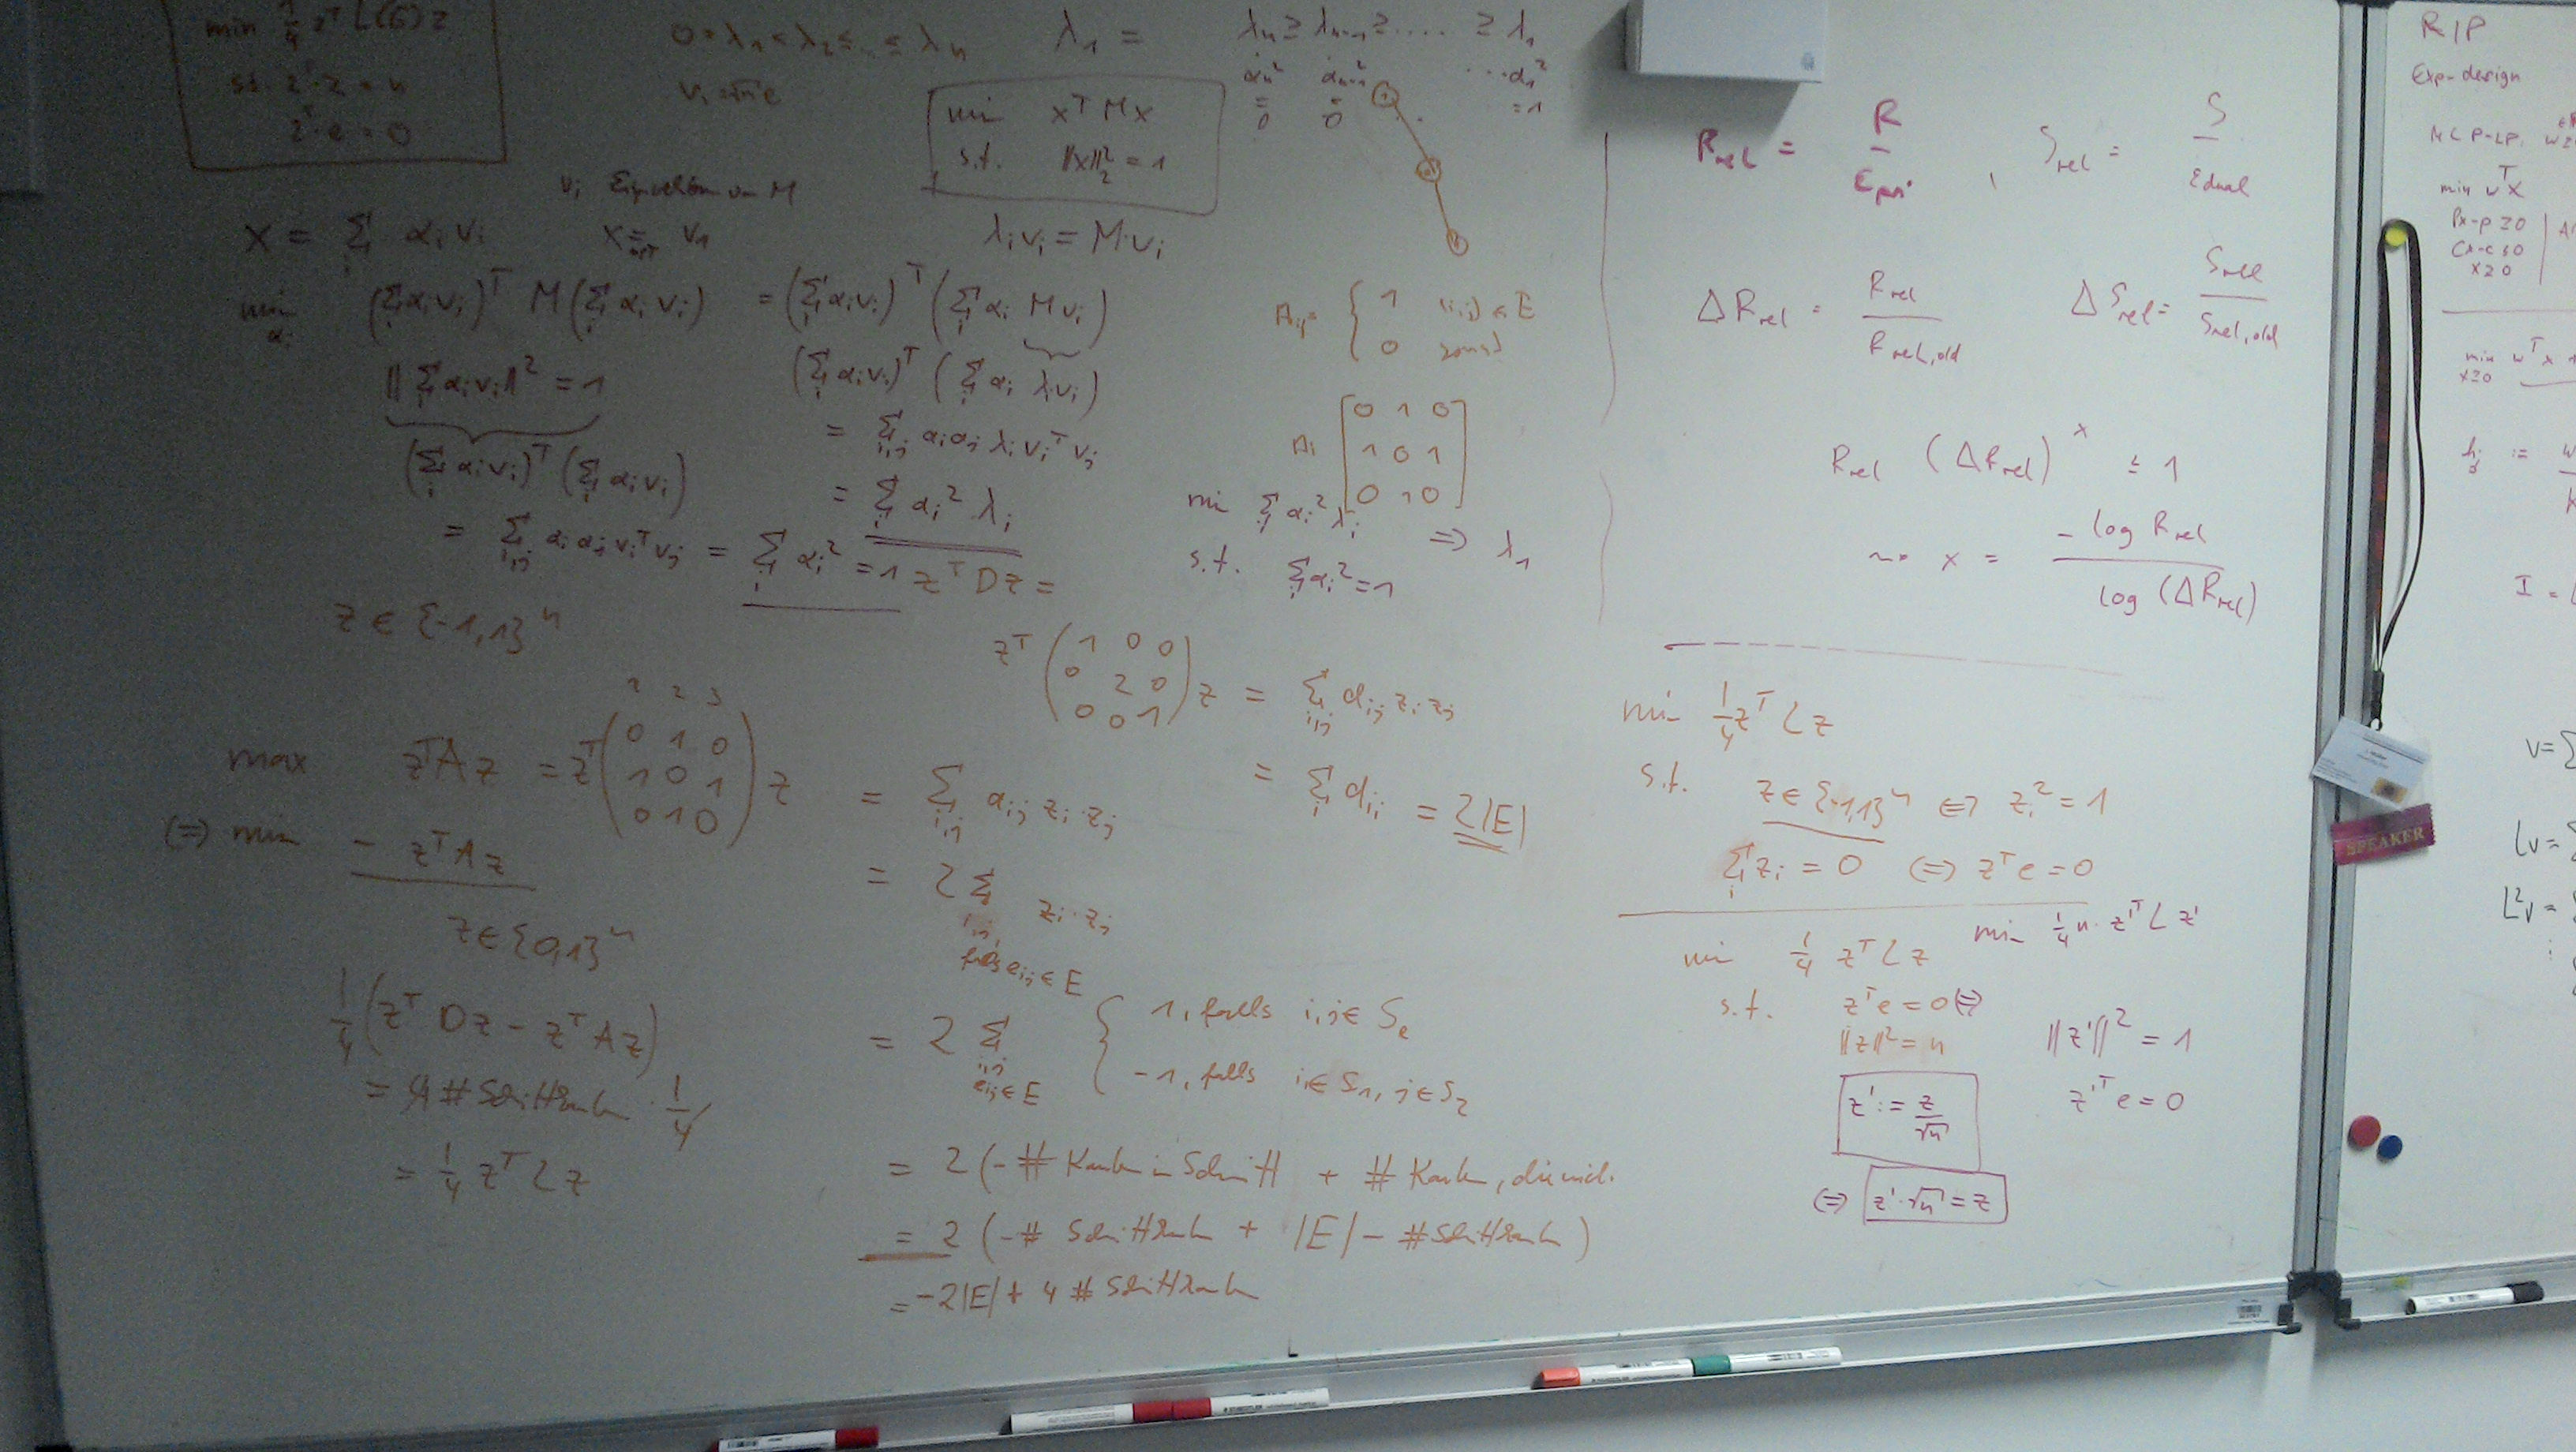
\includegraphics[width=\textwidth]{images/sl.jpg}
		\caption{Herleitung}
		\label{rfidtest_xaxis}
\end{figure}

\begin{mysatz*}
Sei $G=(V,E)$ ein Graph und $V=V_1\cup V_2$ eine Partition, dann gilt:
\begin{itemize}
	\item Die minimale Anzahl an Kanten, welche die beiden Gebiete $V_1$ und $V_2$ verbinden ist mindestens $\dfrac{1}{4}\lambda_2 |V|$, wobei $\lambda_2$ der zweitkleinste Eigenwert von $L(G)$ ist.
	\item Der zu $\lambda_2$ gehörende Eigenvektor $v_2$ heißt Fiedler-Vektor und minimiert das zugehörige Minimierungsproblem.
\end{itemize}
\end{mysatz*}

\subsection{Algorithmus}
\begin{lstlisting}
SpektraleBisektion(V,E):
	Berechne L(G)
	Berechne v2
	Berechne den Median M aller Komponenten von v2
	for v[i] in V:
		if v2[i] < M:
			lege v in V[1]
		if v2[i] >= M:
			lege v in V[2]
\end{lstlisting}
\end{document}
